\section{Functional specification}
\subsection{Introduction}
\paragraph{Smart contract vulnerabilities:}
\begin{itemize}
    \item Unexpected ether flows
    \item Unprivileged writes
    \item Use of unsafe inputs
    \item Reentrant method calls
    \item Transaction reordering
    \item Arithmetic overflows
\end{itemize}{}
\textbf{\color{blue}Unknown unknowns: }Some "cool" quote from Christoph Jentzsch: \textit{We believe more security audits or more tests would have made no difference. The main problem was that reviewers did not know what to look for.}\\
\textbf{The problem: \newline}
\begin{minipage}{0.5\linewidth}
    \centering      
    \def\svgwidth{\linewidth}
    %% Creator: Inkscape inkscape 0.92.4, www.inkscape.org
%% PDF/EPS/PS + LaTeX output extension by Johan Engelen, 2010
%% Accompanies image file 'L6_vulnerabilites_problems.pdf' (pdf, eps, ps)
%%
%% To include the image in your LaTeX document, write
%%   \input{<filename>.pdf_tex}
%%  instead of
%%   \includegraphics{<filename>.pdf}
%% To scale the image, write
%%   \def\svgwidth{<desired width>}
%%   \input{<filename>.pdf_tex}
%%  instead of
%%   \includegraphics[width=<desired width>]{<filename>.pdf}
%%
%% Images with a different path to the parent latex file can
%% be accessed with the `import' package (which may need to be
%% installed) using
%%   \usepackage{import}
%% in the preamble, and then including the image with
%%   \import{<path to file>}{<filename>.pdf_tex}
%% Alternatively, one can specify
%%   \graphicspath{{<path to file>/}}
%% 
%% For more information, please see info/svg-inkscape on CTAN:
%%   http://tug.ctan.org/tex-archive/info/svg-inkscape
%%
\begingroup%
  \makeatletter%
  \providecommand\color[2][]{%
    \errmessage{(Inkscape) Color is used for the text in Inkscape, but the package 'color.sty' is not loaded}%
    \renewcommand\color[2][]{}%
  }%
  \providecommand\transparent[1]{%
    \errmessage{(Inkscape) Transparency is used (non-zero) for the text in Inkscape, but the package 'transparent.sty' is not loaded}%
    \renewcommand\transparent[1]{}%
  }%
  \providecommand\rotatebox[2]{#2}%
  \newcommand*\fsize{\dimexpr\f@size pt\relax}%
  \newcommand*\lineheight[1]{\fontsize{\fsize}{#1\fsize}\selectfont}%
  \ifx\svgwidth\undefined%
    \setlength{\unitlength}{594.2851774bp}%
    \ifx\svgscale\undefined%
      \relax%
    \else%
      \setlength{\unitlength}{\unitlength * \real{\svgscale}}%
    \fi%
  \else%
    \setlength{\unitlength}{\svgwidth}%
  \fi%
  \global\let\svgwidth\undefined%
  \global\let\svgscale\undefined%
  \makeatother%
  \begin{picture}(1,0.26069923)%
    \lineheight{1}%
    \setlength\tabcolsep{0pt}%
    \put(0,0){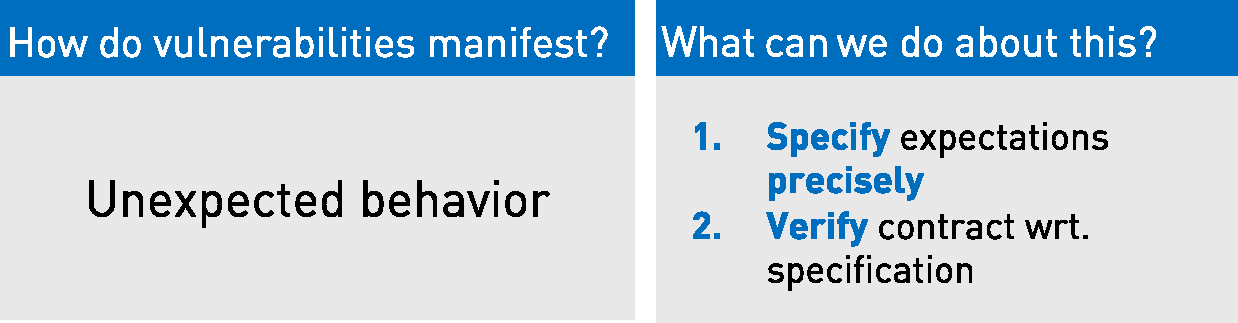
\includegraphics[width=\unitlength,page=1]{Figures/L6_vulnerabilites_problems.pdf}}%
  \end{picture}%
\endgroup%
    
\end{minipage}
TODO WTF?
\subsection{Property Behaviors}
\paragraph{Definitions:}
\begin{itemize}
    \item \textbf{\textcolor{blue}{Execution}} = sequence of function calls
    \item \textbf{\textcolor{blue}{Behavior}} =  corresponding sequence of (message, state) pairs
    \item The set of possible  \textbf{\textcolor{blue}{execution trees}} is defined by the following grammar:\\
    Exec ::= Start$^{\infty}$ \quad Start ::= Call \quad Call::= Msg [ Cmd* ] \quad Cmd ::= Call | ...
    \item A \textbf{\textcolor{blue}{complete call}} of a bundle of contracts is a \textbf{\textcolor{blue}{subtree}} of a valid execution tree such that:
    \begin{enumerate}
        \item the root is a \textbf{\textcolor{blue}{call}} to the bundle
        \item \textbf{\textcolor{blue}{not nested}} in other such call
    \end{enumerate}{}
    \item Every  complete call of the bundle gives rise to an \textbf{\textcolor{blue}{observation of the bundle}} which records:
    \begin{enumerate}
        \item the \textbf{\textcolor{blue}{message}} used  to call the bundle
        \item the \textbf{\textcolor{blue}{bundle state}} right after the call
    \end{enumerate}{}
    \item A \textbf{\textcolor{blue}{property}} w.r.t. \textbf{\textcolor{blue}{the bundle}} is merely a set \textbf{$P$} of infinite observation sequences $\alpha$\\
    Examples:
    \begin{description}
        \item[$P_1$] = \{$\alpha$ : all investments in $\alpha$ get deposited to Escrow\}
        \item[$P_2$] = \{$\alpha$ : all withdrawals in $\alpha$ happen only after the Crowdsale was closed\}
        \item[$P_3$] = \{$\alpha$ : the Crowdsale is eventually closed in $\alpha$\}
    \end{description}{}
\end{itemize}{}
\paragraph{Safety vs Liveness\\}
\begin{multicols}{2}
 \textbf{Safety}  \\ \rule{\linewidth}{0.4pt} \\A safety property requires that something \textbf{\textcolor{blue}{bad never happen}}, e.g., a withdrawal  never happens before a closure. \\ \\ \textbf{Formally:\\}
$P$ is a \textbf{safety} property iff for all infinite $\alpha$
$$
\begin{array}{c}
\alpha \notin P \Leftrightarrow \exists \text { bad } \prec \alpha \forall \beta \in P: \text { bad } \not\prec \beta \\ \\
\textit { Safety } \sim \textit { correctness. }
\end{array}
$$
 \columnbreak 
 \\ \\ \textbf{Liveness}  \\ \rule{\linewidth}{0.4pt}  \\ A liveness property requires that something \textbf{\textcolor{blue}{good happens often enough}}, e.g., the crowdsale eventually closes. \\ \\
\textbf{Formally:}\\
$P$ is a \textbf{liveness} property iff for all finite $\alpha$
$$
\begin{array}{c}
\exists \beta: \alpha \beta \in P \\ \\
\textit {Liveness } \sim \textit {delivery}
\end{array}
$$
\end{multicols}
Examples:
\begin{description}
    \item[$P_1$] = \{$\alpha$ : all investments in $\alpha$ get deposited to Escrow\}
        \begin{enumerate}
            \item[--] \textcolor{blue}{Safety} (depends on English interpretation)
        \end{enumerate}
    \item[$P_2$] = \{$\alpha$ : all withdrawals in $\alpha$ happen only after the Crowdsale was closed\}
    \begin{enumerate}
            \item[--] \textcolor{blue}{Safety}
        \end{enumerate}
    \item[$P_3$] = \{$\alpha$ : the Crowdsale is eventually closed in $\alpha$\}
    \begin{enumerate}
            \item[--] \textcolor{blue}{Liveness}
        \end{enumerate}
\end{description}{}

\subsection{Linear Temporal Logic (LTL)}
\paragraph{Introduction}
Consider the property:
\{$\alpha$ : all withdrawals in $\alpha$ happen only after the Crowdsale was closed\}
\begin{enumerate}
   \item[--] Classical logic definition:\\
        $\varphi(\alpha) \equiv \forall t \in \mathbb{N}: \text { fun }[\alpha | t]]=\text { withdraw } \rightarrow \exists s \leqslant t: \text { fun }[\alpha | s]]=\text { close. }$
    \item[--] LTL definition \\
    $\varphi \equiv \square(\text { fun }=\text { withdraw } \rightarrow \text { Gfun }=\text { close })$
\end{enumerate}{}
\subsection{LTL Syntax}

\begin{multicols}{2}
 \textbf{Terms}  \\ \rule{\linewidth}{0.4pt} \begin{enumerate}
    \item[--] \textbf{\textcolor{blue}{Variables}} (a.k.a. flexible variables) fun, raised, goal, ...
    \item[--] \textbf{\textcolor{blue}{Constants}} (a.k.a. rigid variables) $u, v, w, \ldots, 0,1,2, \ldots$
    \item[--] Application of \textbf{\textcolor{blue}{function symbols}} raised \textbf{\textcolor{blue}{+}} goal, ...
 \end{enumerate}{}
 \\
 \columnbreak 
 \\ \\ \textbf{Formulas}  \\ \rule{\linewidth}{0.4pt}  
 \begin{enumerate}
    \item[--] Application of \textbf{\textcolor{purple}{relation symbols}} fun \textcolor{purple}{$=$} withdraw, raised \textcolor{purple}{$<=$} goal
    \item[--] Application of \textbf{\textcolor{purple}{logical connectives}} $\varphi \textcolor{purple}{\wedge} \psi, \varphi \textcolor{purple}{\vee} \psi, \varphi \textcolor{purple}{\rightarrow} \psi, \ldots$
    \item[--] Application of \textbf{\textcolor{purple}{temporal connectives}}
        $\textcolor{purple}{\square} \varphi, \textcolor{purple}{\diamond}\varphi, \textcolor{purple}{\blacksquare } \varphi, \textcolor{purple}{\diamondsuite} \varphi, \ldots$
 \end{enumerate}{}
 \end{multicols}
 
 TODO filled diamond\\
 filled square = \textbf{so far}
 \begin{minipage}{0.5\linewidth}
    \centering      
    \def\svgwidth{\linewidth}
    %% Creator: Inkscape inkscape 0.92.4, www.inkscape.org
%% PDF/EPS/PS + LaTeX output extension by Johan Engelen, 2010
%% Accompanies image file 'L6_LTL_semantics.pdf' (pdf, eps, ps)
%%
%% To include the image in your LaTeX document, write
%%   \input{<filename>.pdf_tex}
%%  instead of
%%   \includegraphics{<filename>.pdf}
%% To scale the image, write
%%   \def\svgwidth{<desired width>}
%%   \input{<filename>.pdf_tex}
%%  instead of
%%   \includegraphics[width=<desired width>]{<filename>.pdf}
%%
%% Images with a different path to the parent latex file can
%% be accessed with the `import' package (which may need to be
%% installed) using
%%   \usepackage{import}
%% in the preamble, and then including the image with
%%   \import{<path to file>}{<filename>.pdf_tex}
%% Alternatively, one can specify
%%   \graphicspath{{<path to file>/}}
%% 
%% For more information, please see info/svg-inkscape on CTAN:
%%   http://tug.ctan.org/tex-archive/info/svg-inkscape
%%
\begingroup%
  \makeatletter%
  \providecommand\color[2][]{%
    \errmessage{(Inkscape) Color is used for the text in Inkscape, but the package 'color.sty' is not loaded}%
    \renewcommand\color[2][]{}%
  }%
  \providecommand\transparent[1]{%
    \errmessage{(Inkscape) Transparency is used (non-zero) for the text in Inkscape, but the package 'transparent.sty' is not loaded}%
    \renewcommand\transparent[1]{}%
  }%
  \providecommand\rotatebox[2]{#2}%
  \newcommand*\fsize{\dimexpr\f@size pt\relax}%
  \newcommand*\lineheight[1]{\fontsize{\fsize}{#1\fsize}\selectfont}%
  \ifx\svgwidth\undefined%
    \setlength{\unitlength}{648.0000173bp}%
    \ifx\svgscale\undefined%
      \relax%
    \else%
      \setlength{\unitlength}{\unitlength * \real{\svgscale}}%
    \fi%
  \else%
    \setlength{\unitlength}{\svgwidth}%
  \fi%
  \global\let\svgwidth\undefined%
  \global\let\svgscale\undefined%
  \makeatother%
  \begin{picture}(1,0.59115184)%
    \lineheight{1}%
    \setlength\tabcolsep{0pt}%
    \put(0,0){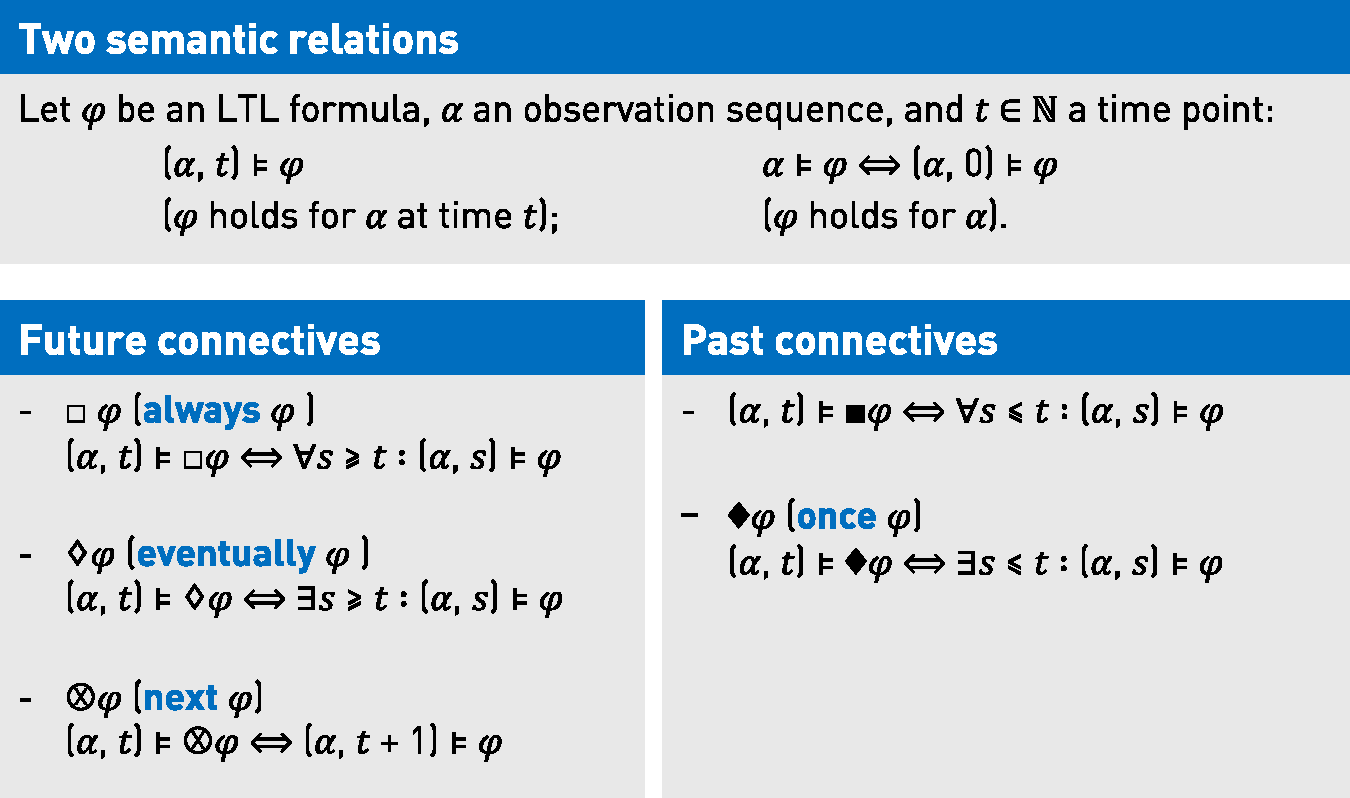
\includegraphics[width=\unitlength,page=1]{Figures/L6_LTL_semantics.pdf}}%
  \end{picture}%
\endgroup%
    
\end{minipage}


\begin{multicols}{2}
 \textbf{Constants (a.k.a. rigid variables)}  \\ \rule{\linewidth}{0.4pt} \\
 A constant $u$ may vary in time only w.r.t. surrounding temporal connectives:
 \begin{description}
    \item[LTL:] $\quad \square \existsu:(cl=u) \wedge \otimes(c l=u+1)]$
    \item[Classical:] $ \forall t \in \mathbb{N}: \exists u: \operatorname{cl}[t]=u \wedge c\lfloor[t+1]=u+1$
\end{description}{}
 \columnbreak 
 \\ \\ \textbf{Variables (a.k.a. flexible variables)}  \\ \rule{\linewidth}{0.4pt}  \\
 A variable u may vary in time freely: 
 \begin{description}
     \item[LTL:] $\square \exists u:(\mathrm{cl}=u) \wedge \otimes(c l=u+1))$
     \item[Classical:] $\forall t \in \mathbb{N}: \exists u: \mathrm{cl}[t]=\mathrm{u}[t] \wedge \mathrm{cl}[t+1]=\mathrm{u}[t+1]+1$
 \end{description}{}
 \end{multicols}
 \paragraph{Duality: De Morgan’s laws}
 \begin{minipage}{0.5\linewidth}
    \centering      
    \def\svgwidth{\linewidth}
    %% Creator: Inkscape inkscape 0.92.4, www.inkscape.org
%% PDF/EPS/PS + LaTeX output extension by Johan Engelen, 2010
%% Accompanies image file 'L6_LTL_semantics.pdf' (pdf, eps, ps)
%%
%% To include the image in your LaTeX document, write
%%   \input{<filename>.pdf_tex}
%%  instead of
%%   \includegraphics{<filename>.pdf}
%% To scale the image, write
%%   \def\svgwidth{<desired width>}
%%   \input{<filename>.pdf_tex}
%%  instead of
%%   \includegraphics[width=<desired width>]{<filename>.pdf}
%%
%% Images with a different path to the parent latex file can
%% be accessed with the `import' package (which may need to be
%% installed) using
%%   \usepackage{import}
%% in the preamble, and then including the image with
%%   \import{<path to file>}{<filename>.pdf_tex}
%% Alternatively, one can specify
%%   \graphicspath{{<path to file>/}}
%% 
%% For more information, please see info/svg-inkscape on CTAN:
%%   http://tug.ctan.org/tex-archive/info/svg-inkscape
%%
\begingroup%
  \makeatletter%
  \providecommand\color[2][]{%
    \errmessage{(Inkscape) Color is used for the text in Inkscape, but the package 'color.sty' is not loaded}%
    \renewcommand\color[2][]{}%
  }%
  \providecommand\transparent[1]{%
    \errmessage{(Inkscape) Transparency is used (non-zero) for the text in Inkscape, but the package 'transparent.sty' is not loaded}%
    \renewcommand\transparent[1]{}%
  }%
  \providecommand\rotatebox[2]{#2}%
  \newcommand*\fsize{\dimexpr\f@size pt\relax}%
  \newcommand*\lineheight[1]{\fontsize{\fsize}{#1\fsize}\selectfont}%
  \ifx\svgwidth\undefined%
    \setlength{\unitlength}{487.35001211bp}%
    \ifx\svgscale\undefined%
      \relax%
    \else%
      \setlength{\unitlength}{\unitlength * \real{\svgscale}}%
    \fi%
  \else%
    \setlength{\unitlength}{\svgwidth}%
  \fi%
  \global\let\svgwidth\undefined%
  \global\let\svgscale\undefined%
  \makeatother%
  \begin{picture}(1,0.47466527)%
    \lineheight{1}%
    \setlength\tabcolsep{0pt}%
    \put(0,0){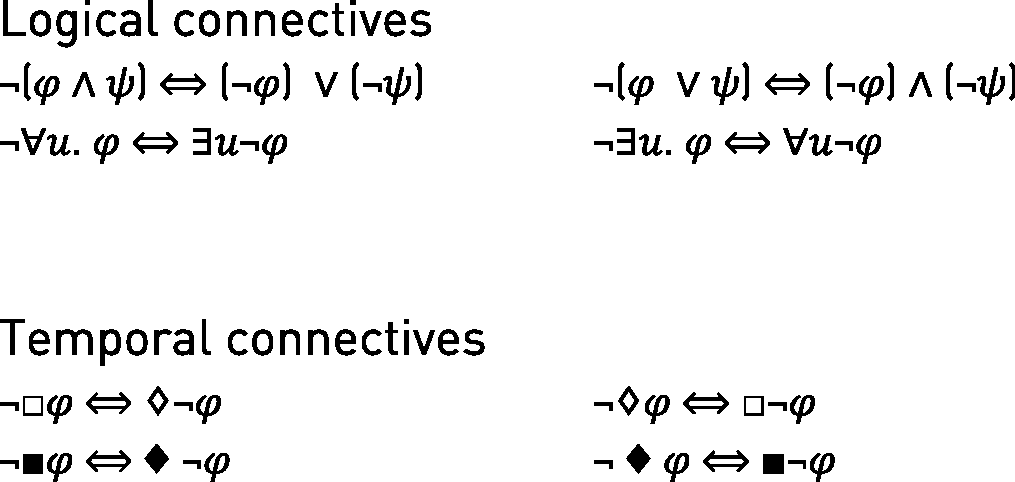
\includegraphics[width=\unitlength,page=1]{Figures/L6_LTL_demorgan.pdf}}%
  \end{picture}%
\endgroup%
    
\end{minipage}

\paragraph{Theorems:}
\begin{enumerate}
    \item[] If $\varphi$ is a non-temporal formula (no temporal connectives), $\square \varphi$ defines a safety property.
    \item[] If $\varphi$ be a past formula (no future connectives), $\square \varphi$ defines a safety property. Also known as \textbf{Canonical Safety}
\end{enumerate}{}
